\section{Case Study}\label{sec:case-study}

\subsection{Case Study Design}

In order to identify the architectural differences between implementations of microservice architectures implemented with REST and GraphQL interfaces, a case study is performed.
To be independent of past design decisions, the case study is performed on a newly implemented example project.

The example project implements the setting of an online shop as shown in \autoref{fig:cs-setting}.
The shop keeps its inventory in one or more warehouses.
When the user orders items from the shop, the inventory is checked and the ordered items are reserved.
When the user's bank processes the payment to the shop, the reserved items of the order are shipped to the user.
For this case study, the user's payment instruction to their bank, and the bank's processing of the payment is outside of the scope.

\begin{figure}[!htb]
    \centering
    \begin{tikzpicture}[
    node distance=3cm,
    comp/.style = {
        draw,
        circle,
        text width = 2cm,
        align = center,
        thick
    },
    l/.style = {
        text width = 3cm
    }
]

\node[comp] (user) {User};
\node[comp, rectangle, right=of user] (shop) {Shop};
\node[comp, rectangle, right=of shop] (ware) {Warehouse};
\node[comp, rectangle, below=of user] (bank) {Bank};
\node[comp, rectangle, below=of ware] (post) {Postal Service};

\draw[->, thick] (user) -- node[above, l, align=center] {orders items} (shop);
\draw[->, thick] (user) -- node[right, l, yshift=.5cm] {instructs payment} (bank);

\draw[->, thick] (shop) -- node[above, l, align=center] {checks inventory \& reserves items} (ware);
\draw[->, thick] (shop) -- node[right, l] {ships items} (post);

\draw[->, thick] (bank) -- node[right, l] {sends payment} (shop);

\draw[dashed] ($(user)!0.5!(shop)$) + (0, 1cm) -- +(0, -5cm);

\end{tikzpicture}
    \caption{Setting of the Case-Study}\label{fig:cs-setting}
\end{figure}

In the first step of the case study, this setting is implemented twice with a microservice architecture, first using \ac{REST} and then using GraphQL.% checktex 13
After implementing the case study, the architecture of both implementations is compared.
At this point, a service cut was intentionally not defined to evaluate if the different technologies also suit a different service cut.

Using both implementations of this scenario, the performance can be compared.
This can be done by defining a set of request scenarios (e.g.~a user orders 5 items and pays immediately afterward).
The resulting load on the system can then be measured in two different ways.
First, the average response time until a user's request is executed can be measured.
This is important as fast processing of requests is essential to a user's experience of using the system.
Second, the generated load on the internal network connecting the microservices can be measured.
While this case study only utilizes a single network, for geographically distributed microservices, the network can be a bottleneck.

The last part of the case study is to evaluate a schema evolution of the data held by the microservices.
This step consists of introducing the additional constraint, that the shipping cost of an order is now dependant on the weight of the items.
This means, that each item now has an additional property, which is consumed within the system.

\subsection{Implementation of \acs{REST} Microservices}

To implement the case study using a \ac{REST} \ac{API} for communication between the microservices, a service cut consisting of four different services was chosen.

\paragraph{Inventory Service}

The inventory service manages the available \textit{items}, and where they are stored.
It maintains a set of \textit{warehouses} where items are located.
Items and warehouses are associated with each other by \textit{stock positions}.
While the items themselves maintain only information such as name or price, stock positions maintain how many of one item is stored in a warehouse.
Additionally, each stock position stores how many of an item in the warehouse is available.
In this case, an item is available, if it is not yet part of an existing order.

\paragraph{Order Service}

The order service accepts the user's \textit{orders}.
When a new order is created, the service first verifies that for each \textit{position of the order} enough items are in stock to fulfill the order.
This is done by requesting the stock positions of the items from the inventory service.
If enough items are available, the items are reserved (marked as unavailable).
Next, the shipping service is contacted to calculate the shipping cost for the order and to create a new shipment.
The total of the order is calculated and the payment service is instructed to create a payment with the calculated sum.
The order service is the main service, users interact with.
Apart from that, it provides endpoints to the other services to update the status of the order (i.e. \textit{payment received} or \textit{shipped}).

\paragraph{Shipping Service}

The shipping service manages \textit{shipments} for orders.
In this case study, it only calculates the cost of shipping for an order.
In a real-world implementation, this service could additionally interface with third-party \acp{API} of postal services and print labels for the packages.

\paragraph{Payment Service}

The payment service manages \textit{payments} for orders.
Similarly to the shipping service, this service only stores the due amount, but could interface with payment processors in a real-world setting.


A complete overview of the interaction of the services is shown in \autoref{fig:interaction}.
The user creates a new order~\raisebox{.5pt}{\textcircled{\raisebox{-.9pt} {1}}}, the order service checks if enough items are in stock~\raisebox{.5pt}{\textcircled{\raisebox{-.9pt} {2}}} and reserves the items if they are~\raisebox{.5pt}{\textcircled{\raisebox{-.9pt} {3}}}.
Then, a new shipment is created by the shipping service~\raisebox{.5pt}{\textcircled{\raisebox{-.9pt} {4}}} and a new payment is created by the payment service~\raisebox{.5pt}{\textcircled{\raisebox{-.9pt} {5}}}.
When the payment is received~\raisebox{.5pt}{\textcircled{\raisebox{-.9pt} {6}}}, the order is updated~\raisebox{.5pt}{\textcircled{\raisebox{-.9pt} {7}}} and the shipping service is instructed to ship it~\raisebox{.5pt}{\textcircled{\raisebox{-.9pt} {8}}}.
Finally, the items are booked out from the inventory~\raisebox{.5pt}{\textcircled{\raisebox{-.9pt} {9}}}.

\begin{figure}[!htb]
    \centering
    \begin{tikzpicture}[
    node distance=3cm,
    comp/.style = {
        draw,
        circle,
        text width = 2cm,
        align = center,
        thick
    },
    l/.style = {
        text width = 3cm
    }
]

\node[comp, color=theme5, fill=theme5!10!white] (order) {Order Service};
\node[comp, below=of order, color=theme1, fill=theme1!10!white] (payment) {Payment Service};
\node[comp, above=of order, color=theme3, fill=theme3!10!white] (inventory) {Inventory Service};
\node[comp, right=of order, color=theme2, fill=theme2!10!white] (shipping) {Shipping Service};

\node[comp, left=of order] (client) {Client};
\node[comp, left=of payment] (paymentProcessor) {Payment Processor};

\draw[->, thick] (client) -- node[l, above, align=center] {\raisebox{.5pt}{\textcircled{\raisebox{-.9pt} {1}}} create order} (order);
\draw[->, thick] (order) to [bend left] node[l, left, align=right] {\raisebox{.5pt}{\textcircled{\raisebox{-.9pt} {2}}} check stock} (inventory);
\draw[->, thick] (order) to [bend right] node[l, right, align=left] {\raisebox{.5pt}{\textcircled{\raisebox{-.9pt} {3}}} reserve item} (inventory);
\draw[->, thick] (order) to [bend left] node[l, above, align=center] {\raisebox{.5pt}{\textcircled{\raisebox{-.9pt} {4}}} create shipment} (shipping);
\draw[->, thick] (order) to [bend right] node[l, left, align=right] {\raisebox{.5pt}{\textcircled{\raisebox{-.9pt} {5}}} create payment} (payment);
\draw[->, thick] (paymentProcessor) -- node[l, above, align=center] {\raisebox{.5pt}{\textcircled{\raisebox{-.9pt} {6}}} payment information} (payment);
\draw[->, thick] (payment) to [bend right] node[l, right, align=left] {\raisebox{.5pt}{\textcircled{\raisebox{-.9pt} {7}}} update order} (order);
\draw[->, thick] (order) to [bend right] node[l, below, align=center] {\raisebox{.5pt}{\textcircled{\raisebox{-.9pt} {8}}} ship order} (shipping);
\draw[->, thick] (shipping) to [bend right] node[l, right, align=left, text width=3.2cm] {\raisebox{.5pt}{\textcircled{\raisebox{-.9pt} {9}}} book out items} (inventory);

\end{tikzpicture}
    \caption{Service Interactions}\label{fig:interaction}
\end{figure}

\subsubsection{Technology Stack}\label{sec:rest-tech}

Each \acs{REST} microservice was implemented using the general-purpose programming language Java, and the Spring framework\footnote{\url{https://spring.io}}.
Findings of Schermann~\cite{Schermann2015} show, that Java is the most commonly used programming language for microservices.
Spring is a widely used framework for enterprise applications.
According to Snyk's annual \acs{JVM} Ecosystem Report~\cite{Vermeer2020}, 6 out of 10 \acs{JVM} developers use the Spring framework.
Spring is a modular, open-source framework consisting of a set of libraries providing for example dependency injection, data access, a server-side web framework, or cloud integration.

Each of the services is packaged as a Docker\footnote{\url{https://www.docker.com/}} Linux container.
These containers allow to easily distribute the packaged service and simplify the creation of replicas.
The containers for the microservices expose a port to accept \ac{HTTP} requests, that will be handled by the Spring framework.
However, each container is assigned its own IP address, which makes scaling difficult, as the destination for requests needs to be known beforehand.
Thus, an additional container running Traefik is placed before the microservice containers.
Traefik\footnote{\url{https://containo.us/traefik/}} is a reverse proxy and load balancer designed for microservices and has various integrations with different kinds of infrastructure, such as Docker or Kubernetes.

The microservices use the PostgreSQL\footnote{\url{https://www.postgresql.org/}} database system for data storage.
However, multiple instances of the same microservice share just one instance of a containerized database.
In a real-world deployment, the database should not be containerized at all, but rather a distributed database cluster should be used, to achieve high availability, redundancy, and high performance.
Communication with the database is implemented using the Spring Data \acs{JPA}, which provides convenient access to \ac{JPA} data sources.

\begin{figure}[!htb]
    \centering
    \begin{tikzpicture}[
    node distance=1.25cm,
    container/.style = {
        draw
    },
    application/.style = {
        draw,
        regular polygon,
        regular polygon sides = 4,
        text width=.5cm,
        align = center
    },
    database/.style = {
        draw,
        cylinder,
        shape border rotate=90,
        aspect=0.25,
        text width = .5cm,
        minimum height = 1cm,
        align = center%,
        %cylinder uses custom fill, cylinder body fill=white, cylinder end fill=black!5
    },
]

\node[draw, text width=3cm, align=center, minimum height=1cm] (traefik) {
\includegraphics[width=.5cm,page=1]{images/image.pdf}\\ Reverse Proxy};

\draw[->] ($(traefik)+(0,1.5cm)$) -- node[above,yshift=.25cm,text width=5cm,align=center] {\acs{HTTP} requests\\(external and internal)} (traefik);

\node[application, color=theme5, fill=theme5!10!white, below=1.5cm of traefik] (order1) {O};
\node[application, color=theme5, fill=theme5!10!white, left=of order1] (order2) {O};
\node[application, color=theme3, fill=theme3!10!white, left=of order2] (inventory) {I};
\node[application, color=theme1, fill=theme1!10!white, right=of order1] (payment) {P};
\node[application, color=theme2, fill=theme2!10!white, right=of payment] (shipping) {S};

\draw[->] (traefik) -| node[right, yshift=-1cm] {\footnotesize\texttt{/inventory/*}} (inventory);
\draw[->] (traefik) -- (order1);
\draw[->] (traefik) -- ($(traefik)!0.5!(order1)$) -| node[above, xshift=1.25cm] {\footnotesize\texttt{/order/*}} (order2);
\draw[->] (traefik) -| node[right, yshift=-1cm] {\footnotesize\texttt{/payment/*}} (payment);
\draw[->] (traefik) -| node[right, yshift=-1cm] {\footnotesize\texttt{/shipping/*}} (shipping);

\node[database, color=theme3, fill=theme3!10!white, below=of inventory] (invDb) {};
\node[database, color=theme1, fill=theme1!10!white, below=of payment] (payDb) {};
\node[database, color=theme2, fill=theme2!10!white, below=of shipping] (shipDb) {};
\node[database, color=theme5, fill=theme5!10!white, below=of $(order1.south)!0.5!(order2.south)$] (ordDb) {};

\draw[->] (inventory) -- (invDb);
\draw[->] (order1) |- (ordDb);
\draw[->] (order2) |- (ordDb);
\draw[->] (payment) -- (payDb);
\draw[->] (shipping) -- (shipDb);

\end{tikzpicture}
    \caption{Containers for the \acs{REST} Microservice Architecture}\label{fig:rest-containers}
\end{figure}

A deployment with two Order microservices is shown exemplary in \autoref{fig:rest-containers}.
Traefik accepts all \ac{HTTP} requests --- regardless whether they come directly from users, or other microservices --- and routes them to the appropriate microservice depending on the so-called context path.
The context path specifies a path prefix in the request \ac{URL} and Traefik can be configured to route certain prefixes to certain types of services.
This configuration happens through labels on Docker containers, which can be used to apply metadata to them.


\begin{lstlisting}[caption={Traefik Configuration for the Inventory Service}, showlines=true, label=lst:traefik-docker, language=yaml]
labels:
  - "traefik.enable=true"
  - "traefik.http.routers.inventory.rule=PathPrefix(`/inventory/`)"
  - "traefik.http.routers.inventory.entrypoints=web"
\end{lstlisting}

\autoref{lst:traefik-docker} shows an excerpt of the configuration of the labels for the inventory service.
The labels configure Traefik to route all requests on the \texttt{web} entrypoint with the path prefix \texttt{/inventory/} to this service.
Entrypoints can be configured at Traefik's startup and specify on which port Traefik should listen and can also be configured with different options.
For example, an endpoint could be configured to terminate \ac{TLS} connections and forward the requests without encryption to the appropriate backend service.

\subsubsection{\acs{API} Style}

For the first part of the case study, the \ac{REST} architectural style mandated a resource-based \ac{API} style~\cite{Fielding2000}.
This means, that the services expose their resources at unique \acp{URL}.
All endpoints produce \ac{JSON} following the \ac{HAL} format.

For example, the inventory service provides the endpoints in \autoref{tab:endpoints-inv-items} for manipulating stock positions of an item.
Similar to paths in a file system, the trailing slash indicates that the resource is a collection of items, while no trailing slash indicates that a single resource is returned.


\begin{table}[ht]
    \centering
    \begin{tabular}{@{}lll@{}}
        \toprule
        \textbf{Endpoint}                                   & \textbf{\acs{HTTP} Methods} \\
        \midrule
        \texttt{/api/v1/item/\{itemId\}/stock/}             & \texttt{GET}, \texttt{POST} \\
        \texttt{/api/v1/item/\{itemId\}/stock/\{stockId\}}  & \texttt{GET}, \texttt{PUT}, \texttt{DELETE} \\
        \bottomrule
    \end{tabular}
    \caption{Endpoints for Item Resources of the Inventory Service}\label{tab:endpoints-inv-items}
\end{table}

The \texttt{GET} method on the first endpoint fetches a collection of stock positions of the item with the given identifier.
It supports the optional query parameters \texttt{page} and \texttt{size}, to implement pagination and to avoid loading all resources when only a few are needed.
The \texttt{POST} method on the collection is implemented with the semantics of creating a new stock position and adding it to the collection.
This create operation was intentionally implemented using this method, as its semantics are defined very vaguely by the \ac{HTTP} specification~\cite{RFC7321}.
However, using the \texttt{PUT} method would not be appropriate, because its semantics are defined to be replacing the current representation of the resource with the one in the request.
The methods on the second endpoint are implemented to conform to the \ac{HTTP} specification by returning, replacing, and deleting the requested resource respectively.

As an example, a response to a \texttt{GET} request to a stock position resource is shown in \autoref{lst:response-stock-pos}.
The response is the \ac{JSON} representation of the position, containing information about how much items are in stock and how much items are available for sale.

\begin{lstlisting}[caption={Response to Fetching the Stock Position Collection}, language=json, label={lst:response-stock-pos}]
{
  "inStock": 20,
  "available": 0,
  "_links": {
    "self": { "href": "[...]/api/v1/item/2/stock/3" },
    "item": { "href": "[...]/api/v1/item/2" },
    "warehouse": { "href": "[...]/api/v1/warehouse/1" }
  }
}
\end{lstlisting}

Additionally, the field \texttt{\_links} defined by \ac{HAL} is included for navigating the pagination.
All responses of the \ac{REST} \ac{API} include a certain set of links to related resources depending on the requested resource.
The available link relations for each resource are shown in \autoref{tab:link-types}, however, every resource additionally possesses a link with the relation \texttt{self}, which is the URL of the requested resource.
The collection resource in the table below represents zero or more resources of the other types.
Since this type of resource implements pagination, the link relations it implements can be used to navigate back and forth in the pages of the collection.
All other resource types possess links to subresources, or to related resources of the same or different services.

\begin{table}[ht]
    \centering
    \begin{tabular}{@{}ll@{}}
        \toprule
        \textbf{Resource}   & \textbf{Link Types} \\
        \midrule
        Collections         & \texttt{first}, \texttt{previous}, \texttt{next}, \texttt{last} \\
        \midrule
        Items               & \texttt{stock} \\
        Stock Positions     & \texttt{item}, \texttt{warehouse} \\
        Warehouses          & --- \\
        \midrule
        Orders              & \texttt{status}, \texttt{shipment}, \texttt{payment} \\
        \midrule
        Payments            & \texttt{order}, \texttt{status} \\
        \midrule
        Shipment            & \texttt{order}, \texttt{status}, \texttt{cost} \\
        \bottomrule
    \end{tabular}
    \caption{Link Relations of Resources in the \ac{REST} \ac{API} (without \texttt{self} Relation)}\label{tab:link-types}
\end{table}

Note, that the representation of the resource does not include an explicit identifier field, although it possesses one in the database model.
This is an explicit choice due to the \ac{HATEOAS} model because the identifier of resources can be seen as the \ac{URL} of a resource, which is included as the link of relation type \texttt{self} in \ac{API} responses.
The other links relations provided in the \ac{API} responses allow the client to explore the application state space.
Rather than making client-side assumptions about the application state, the \ac{API} explicitly exposes related resources, that the client might manipulate to achieve its goal.
As a consequence of this, clients do not need to manually construct \acp{URL} of the \ac{API} as they are already included in its responses.

\begin{figure}[!htb]
    \centering
    \begin{tikzpicture}[
    node distance=0.5cm,
    state/.style = {
        rectangle,
        draw,
        align = center,
        rounded corners=5mm,
        minimum height = 1cm,
        text width = 2cm
    },
    sync/.style = {
        rectangle,
        fill=black,
        minimum height=1mm,
        minimum width=2cm
    },
    start/.style = {
        circle,
        fill=black
    },
    end/.style = {
        start,
        minimum width = 2mm
    },
    .>/.style = {
        ->,
        dashed
    }
]

\node[start] (ostart) {};
\node[state, below=of ostart] (ocreate) {created};
\draw[->] (ostart) -- (ocreate);

\node[start, right=4cm of ocreate] (pstart) {};
\node[start, left=4cm of ocreate] (sstart) {};
\draw[.>] (ocreate) -- (pstart);
\draw[.>] (ocreate) -- (sstart);

\node[state, below=of pstart] (pcreated) {created};
\draw[->] (pstart) -- (pcreated);

\node[state, below=of pcreated] (ppayed) {payed};
\draw[->] (pcreated) -- (ppayed);

\node[state] at (ocreate |- ppayed) (opayed) {payment received};
\draw[->] (ocreate) -- (opayed);
\draw[.>] (ppayed.west) -- +(-5mm, 0) |- ($(ocreate)!0.5!(opayed)$);

\node[state, below=of sstart] (screated) {created};
\draw[->] (sstart) -- (screated);

\node[state, below=of screated] (sready) {ready to ship};
\draw[->] (screated) -- (sready);
\draw[.>] (opayed.west) -- +(-5mm, 0) |- ($(screated)!0.5!(sready)$);

\node[state, below=of sready] (sshipped) {shipped};
\draw[->] (sready) -- (sshipped);

\node[state] at (sshipped -| opayed) (oshipped) {shipped};
\draw[->] (opayed) -- (oshipped);
\draw[.>] (sshipped.east) -- +(5mm, 0) |- ($(opayed)!0.5!(oshipped)$);

\node[end, below=of oshipped] (oend) {};
\draw (oend) circle (3mm);
\draw[->] (oshipped) -- ($(oend.north)+(0,1mm)$);

\node[end, below=of sshipped] (send) {};
\draw (send) circle (3mm);
\draw[->] (sshipped) -- ($(send.north)+(0,1mm)$);

\node[end, below=of ppayed] (pend) {};
\draw (pend) circle (3mm);
\draw[->] (ppayed) -- ($(pend.north)+(0,1mm)$);

\node[state, below=of oend] (ocancelled) {cancelled};
\draw[->] (ocancelled) -- ($(oend.south)-(0,1mm)$);

\node[state, below=of send] (scancelled) {cancelled};
\draw[->] (scancelled) -- ($(send.south)-(0,1mm)$);

\node[state, below=of pend] (pcancelled) {cancelled};
\draw[->] (pcancelled) -- ($(pend.south)-(0,1mm)$);

\draw[->] (pcreated.east) -- +( 5mm,0) -- ($(pcancelled.south east) + ( 5mm,-5mm)$) -| (pcancelled);
\draw[->] (screated.west) -- +(-5mm,0) -- ($(scancelled.south west) + (-5mm,-5mm)$) -| (scancelled);
\draw     (sready.west)   -- +(-5mm,0);

\draw[->] (ocreate.300) |- ($(ocreate.south east) + ( 5mm,-5mm)$) -- ($(ocancelled.south east) + ( 5mm,-5mm)$) -| (ocancelled);
\draw     (opayed.east) -- +( 5mm,0);

\draw[.>] (ocancelled.west) -- +(-5mm,0) -- +(-5mm,-15mm) -| ($(scancelled.south west) + (3mm,-5mm)$);
\draw[.>] (ocancelled.east) -| ($(pcancelled.south east) + (-3mm,-5mm)$);

\draw[loosely dashed] ($(ocreate.west) + (-2cm, 2.5cm)$) -- +(0,-11.5cm);
\draw[loosely dashed] ($(ocreate.east) + ( 2cm, 2.5cm)$) -- +(0,-11.5cm);

\coordinate (swimlanes) at ($(ocreate.north) + (0,1.5cm)$);
\node at (swimlanes) {Order};
\node at (screated.north |- swimlanes) {Shipment};
\node at (pcreated.north |- swimlanes) {Payment};

\end{tikzpicture}
    \caption{Status Transitions of Application Domain Objects}\label{fig:entity-status}
\end{figure}
 
Another notable style decision of the \ac{API} is the transition of statuses of objects in the application domain.
The general transitions are shown in the status diagram in \autoref{fig:entity-status}, where the dashed lines indicate service-crossing asynchronous triggers of transitions.

These transitions are implemented using a subresource, that can be accessed using the link with the relation \texttt{status} on the main resource.
This endpoint supports the \ac{HTTP} \texttt{GET} and \texttt{PUT} method, where the first returns the status of the resource, and the second updates the status.
Any update to the status may trigger updates of statuses of resources of the same or other services as described in \autoref{fig:entity-status} above.

\subsubsection{\acl{OAS} and Swagger UI}

\ac{OAS} provides a way to describe the endpoints and functionality of \ac{REST} \acp{API} that is language-agnostic, and understandable by humans and computerts~\cite{OAS}.
It can be used both to document an \ac{API} and to generate code for servers or clients.

In the case study, \ac{OAS} was used to generate documentation and a web interface that allows testing the \ac{API} operations.
Using the springdoc-openapi\footnote{\url{https://github.com/springdoc/springdoc-openapi}} Java library, Java's annotations can be used on handler methods of Spring controllers to automatically generate the \ac{API} specification.
\autoref{lst:oas-annotations} shows how the handler methods of Spring controllers can be annotated to automatically generate the specification.

\begin{lstlisting}[language=java, style=java-ext, caption={Java Annotations to Generate \acf{OAS} from Spring Controllers}, label={lst:oas-annotations}]
@Operation(summary = "Get an item by its id")
@ApiResponse(responseCode = "200", 
    description = "Item found", 
    content = {
        @Content(mediaType = "application/hal+json", 
            schema = @Schema(implementation = Item.class))
})
@ApiResponse(responseCode = "404", 
    description = "Item not found", 
    content = {
        @Content(mediaType = "application/hal+json", 
            schema = @Schema(implementation = ApiError.class))
})
@GetMapping("/{id}")
public ResponseEntity<?> getItem(@PathVariable("id") long id) { 
    /* [...] */ }
\end{lstlisting}

\begin{figure}[!htb]
    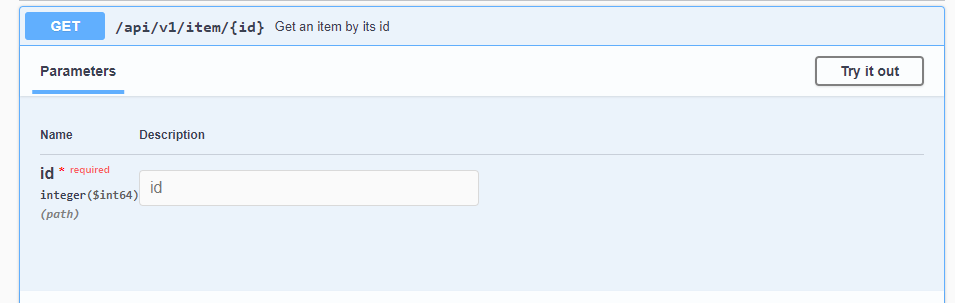
\includegraphics[width=\textwidth]{images/swagger-ui-execute.png}
    \caption{Using SwaggerUI to Execute \ac{API} requests}\label{img:swagger-execute}
\end{figure}

The generated specification can be used together with the web-based tool Swagger UI\footnote{\url{https://swagger.io/tools/swagger-ui/}}.
It can display the specification and the endpoints of the \ac{API} in a graphical format as shown in \autoref{img:swagger-explore}.
However, it can also be used to execute \ac{API} requests and display the result (see \autoref{img:swagger-execute}).
Swagger UI is included for every microservice of the case study and can be used as a graphical way to make requests to the \ac{API} for testing purposes.

\begin{figure}[!htb]
    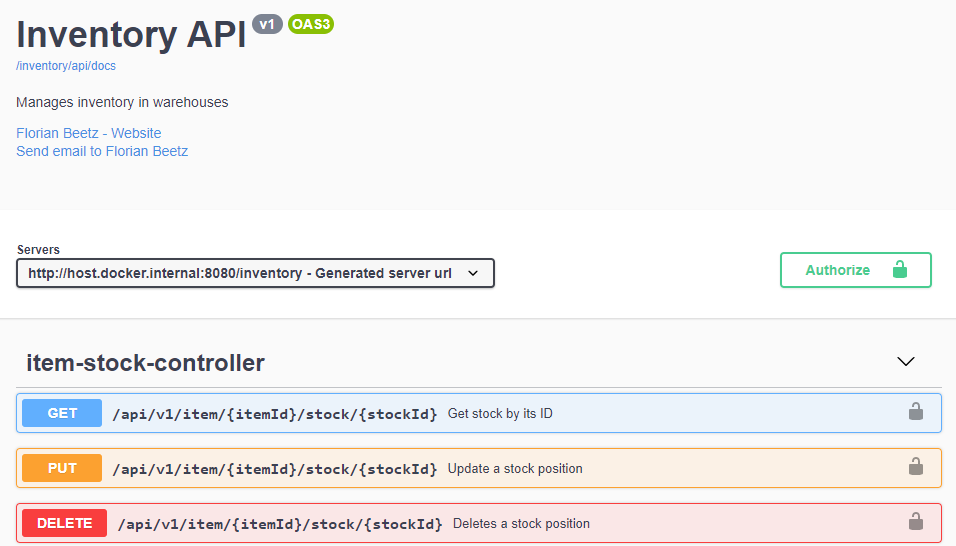
\includegraphics[width=\textwidth]{images/swagger-ui-explore.png}
    \caption{Using SwaggerUI to Explore \ac{API} endpoints}\label{img:swagger-explore}    
\end{figure}

\subsubsection{Client Authentication and Authorization}\label{sec:rest-auth}

In order to implement a mechanism of authenticating users and checking if they are authorized to perform certain operations, \ac{OIDC} was used for the case study.
\ac{OIDC} is a common authentication and authorization scheme used in microservice architectures~\cite{Nehme2019, Hammann2020}.
In general, it can be used to implement \ac{SSO}, delegating authentication and obtaining user information from so-called \acp{IdP} such as Google or Microsoft.
This allows applications to rely on a user's identity provided by a trusted third-party, which is also the reason why these applications are called \acp{RP}.
The \acp{RP} never obtain the credentials of the user, only a token --- usually in the form of a \ac{JWT} --- is provided to them.
This token includes so-called claims, which provide information about the authenticated user, and is signed with the private key of the \ac{IdP}.
Once, a token has been obtained by a \ac{RP}, its authenticity can be verified using the public key of the \ac{IdP}, thus \acp{RP} can be sure that the claims in the token have not been forged.
\autoref{lst:jwt-oidc} shows the payload of a \ac{JWT} by the \ac{IdP} of the \ac{REST} case study.
Each \ac{JSON} field in the payload represent a claim.
While some claims are standardized, in principle any claim can be included in a \ac{JWT}.
Lines one and two specify the expiration timestamp and issuing timestamp respectively.
The \texttt{iss} claim specifies the \ac{URL} of the issuing \ac{IdP} and \texttt{aud} specifies the intended audience of the token.
This information should be verified upon recieval of a token by the service to match the expected values.
The \texttt{Bearer} type specifies, that this token is intended to be sent using the \texttt{Bearer} scheme of \ac{HTTP} authentication.
Line six to eleven then contain the custom claims, first representing the roles the owner of the token has and their username.

\begin{lstlisting}[caption={\ac{JWT} Issued by an \ac{IdP}}, language=json, label={lst:jwt-oidc}]
{ "exp": 1605703187,
  "iat": 1605702887,
  "iss": "http://host.docker.internal:8080/auth/realms/ma-rest-shop",
  "aud": [ "shipping", "payment", "inventory", "order" ],
  "typ": "Bearer",
  "realm_access": {
    "roles": [ "payment_admin", "shipping_admin", "inventory_admin",
          "order_admin", "admin" ]
  },
  [...]
  "preferred_username": "admin"
}
\end{lstlisting}

Using \ac{OIDC} with a own \ac{IdP} makes \ac{OIDC} a suitable authentication mechanism for microservice architectures~\cite{Nehme2019}.
Because tokens and their claims can be verified locally at any service without relying on any external service, this authentication mechanism is easily scalable without introducing a bottleneck and without having to manage credentials locally for services.
The high-level architecture of the authentication mechanism of the case study is shown in \autoref{fig:oidc}.

\begin{figure}[!htb]
    \centering
    \begin{tikzpicture}[
    node distance=1cm,
    component/.style = {
        rectangle,
        draw,
        align = center,
        minimum height = 2cm,
        text width = 2cm
    },
    label/.style = {
        font=\footnotesize\sffamily
    }
]

\node[component] (ua) {Client};

\node[component, below right=of ua] (idp) {Identity Provider};

\node[component, below left= of ua] (svc2) {Service 2};
\node[component, left=of svc2] (svc1) {Service 1};

\draw[->] (ua.west) -| node[above, label, xshift=2cm] {\raisebox{.5pt}{\textcircled{\raisebox{-.9pt} {4}}} authenticated request} (svc1.north);

\draw[->] (ua.30) -| node[above, label, xshift=-1.3cm] {\raisebox{.5pt}{\textcircled{\raisebox{-.9pt} {2}}} authentication} (idp.50);
\draw[->] (idp.130) |- node[above, label, xshift=0.2cm] {\raisebox{.5pt}{\textcircled{\raisebox{-.9pt} {3}}} signed token} (ua.330);

\draw[->] (ua.270) |- node[below, label, text width=3cm, xshift=-0.2cm] {\raisebox{.5pt}{\textcircled{\raisebox{-.9pt} {5}}} authenticated request} (svc2.0);

\draw[->] (svc1.270) -- +(0,-5mm) -| node[below, label, xshift=-5cm] {\raisebox{.5pt}{\textcircled{\raisebox{-.9pt} {1}}} obtain public key} (idp.270);
\draw (svc2.south) -- +(0,-5mm);
\end{tikzpicture}
    \caption{\ac{OIDC} in a Microservice Architecture}\label{fig:oidc}
\end{figure}

First, each service obtains the public key of the \ac{IdP} at startup for token verification.
Then, whenever a client wants to send a request to any service, the user provides their credentials to the \ac{IdP} and obtains a signed token.
Lastly, the obtained token can be used to send authenticated requests to any service.
The services verify the authenticity of the token using the obtained public key of the first step.
If the signature of the token is valid, the services can trust the user to have the roles as claimed in the token.

In order to implement \ac{OIDC} in the \ac{REST} case study, the open-source identity and access management solution Keycloak\footnote{\url{https://www.keycloak.org/}} was used.
Keycloak provides a \ac{SSO} solution out-of-the-box, where applications can implement authentication using \ac{OIDC}, \ac{SAML}, or the basis for \ac{OIDC} OAuth 2.0.
It also provides the ability to broker identities by using public \acp{IdP} providing \ac{OIDC} or \ac{SAML} interfaces.

Using the Keycloak web-interface, a client was created for each service together with one client for external requests.
Clients represent trusted components that are allowed to perform authentication against Keycloak and can specify client-specific roles that can be assigned to users.
Each client defines a role allowing users to perform administrative tasks, such as creating new items for sale or modifying the stock positions of an item.
Additionally, Keycloak allows creating so-called service accounts for each client.
Service accounts can be used to authenticate service-to-service communication and can be assigned roles.
\autoref{tab:roles-rest} shows the available roles for the case study and which service accounts hold which roles.
Note, that assigning the administrative role of a service to itself is unnecessary because the service does not need to make any requests to perform administrative tasks.

\begin{table}[!htb]
    \centering
    \begin{tabular}{@{}lcccc@{}}
        \toprule
        \multirow{2}{*}{\textbf{Role}}  & \multicolumn{4}{c}{\textbf{Service Accounts}} \\
                                        & Inventory & Order & Payment   & Shipping      \\
        \midrule
        \texttt{inventory\_admin}       & ---       & x     &           & x             \\
        \texttt{order\_admin}           &           & ---   & x         & x             \\
        \texttt{payment\_admin}         &           & x     & ---       &               \\
        \texttt{shipping\_admin}        &           & x     &           & ---           \\
        \bottomrule
        
    \end{tabular}
    \caption{Available Roles for the \ac{REST} Case Study and Service Account Association}\label{tab:roles-rest}
\end{table}

Administrative endpoints of the case study project are secured by using the Spring Security\footnote{\url{https://spring.io/projects/spring-security}} library.
Spring Security provides authentication and authorization, but also can be used to mitigate attacks like session fixation or \ac{CSRF}.
It was set up to extract user details from any request if they are available, but to generally allow any request.
Some endpoints that require special privileges are annotated as shown in \autoref{lst:endpoint-sec} to require certain roles.
If a request is sent to such an endpoint without an access token of the \ac{IdP} or the user does not have this role, Spring Security responds with the \ac{HTTP} status codes 401 Unauthorized or 403 Forbidden respectively.

\begin{lstlisting}[caption={Securing \ac{REST} Endpoints using Spring Security}, style=java-ext, label={lst:endpoint-sec}]
@Secured("ROLE_inventory_admin")
@PostMapping("/")
public ResponseEntity<Item> createItem(@RequestBody Item item) {
    /* ... */
}
\end{lstlisting}

\subsubsection{Service-to-Service Communication}

One of the most important properties of microservices is them communicating with each other to provide meaningful features to an end-user.
In the case study, this was implemented by configuring each service with the base \ac{URL} of services it depends on~\cite{Taibi2020}.
While it would be possible for the services to communicate with each other directly over the internal Docker network the containers are running in, the case study implements a different approach.
As already shown in \autoref{sec:rest-tech}, all services communicate only with the reverse proxy.
This approach has several advantages:
First, the microservices do not need to be run inside containers but can also be deployed directly on hardware and second, the reverse proxy can also act as a load-balancer.
This allows for more fine-grained control over how the load is distributed among the instances of a service, however, it also introduces a bottleneck at the load-balancer.

An alternative to this approach would be to implement client-side load-balancing, for example with the Spring Cloud Netflix\footnote{\url{https://github.com/spring-cloud/spring-cloud-netflix}} framework.
This approach would introduce a central service registry, where services would register themselves upon startup.
When a request to another service is to be sent, the registry would be queried for an available instance of the required service.
This would allow pointing services to instances of the required service that are experiencing low load, and load-balancer in front of the instances would not be needed.

Since the \acp{API} of the services are documented with \ac{OAS}, it would be possible to automatically generate clients, for example by using Open\ac{API} Generator\footnote{\url{https://openapi-generator.tech/}}.
However, a different approach was chosen for the case study.
The Spring Framework already provides means of accessing \ac{HTTP} \acp{API} with the \texttt{RestTemplate} \ac{API} and also an implementation for \acp{API} secured with OAuth 2 or \ac{OIDC} with \texttt{OAuth2RestTemplate}.
This implementation automatically obtains access tokens (see \autoref{sec:rest-auth}) and refreshes them when they are expired.
For the case study, this is set up to use the credentials for service accounts of the microservice sending the request.

Another advantage of manually implementing \ac{API} clients results from the use of \ac{HAL}.
Typically, \ac{API} generators use static \acp{URL} for sending requests to endpoints, however, when using \ac{HAL}, the \acp{URL} of the included links object in \ac{API} responses should be used for navigating the \ac{API} operations.
Using this implementation style for clients requires that only a few \acp{URL} need to be constructed because most operations can be discovered from previous communication when another service as shown in \autoref{lst:rest-url-usage}.

\begin{lstlisting}[caption={Updating Shipment Statuses is Implemented Using Link Relations}, style=java-ext, label={lst:rest-url-usage}]
public void setShipmentStatus(Shipment shipment, ShippingStatus status) {
    // ...
    val headers = new HttpHeaders();
    headers.setIfMatch(etag);
    val putResponse = restTemplate.exchange(
        shipment.getRequiredLink(STATUS_RELATION).getHref(), 
        HttpMethod.PUT, 
        new HttpEntity<>(status.name(), headers), 
        Object.class);
    // ...
}
\end{lstlisting}

Following the decentralization principles of microservices, each service has its own implementation of the \ac{API} clients, depending on the needed features.
For example, the client for the inventory \ac{API} of the order service needs to be able to obtain the amount of items in stock, to check if an order can be fulfilled, which is not necessary for the client of the shipping service, which only needs to book out items from the inventory, once they have shipped.
\autoref{tab:ops} shows, which operations are implemented by which client.
The dagger~$\dagger$ denotes, that the operation is used to implement more high-level operations by the client, but can not be accessed explicitly by consumers of the client.
For example, this is the case for the \texttt{getOrderStatus} operation in the implementation of the payment service.
In this instance, the operation is solely used to obtain the current status of the order resource to be able to correctly update it as will be explained in \autoref{sec:http-locking}.

\begin{table}[!htb]
    \centering
    \begin{tabular}{@{}llcccc@{}}
        \toprule
        \multirow{2}{*}{\textbf{\ac{API}}}  & \multirow{2}{*}{\textbf{Operation}}   & \multicolumn{4}{c}{\textbf{Supported by Client of Service}} \\
                                            &                                       & Inventory & Order     & Payment   & Shipping \\
        \midrule
        \multirow{11}{*}{Inventory}         & \texttt{getStock}                     & ---       & $\dagger$ &           & $\dagger$ \\
                                            & \texttt{updateStock}                  & ---       & $\dagger$ &           & $\dagger$ \\
                                            & \texttt{deleteStock}                  & ---       &           &           & \\
                                            & \texttt{getStockOfItem}               & ---       & x         &           & \\
                                            & \texttt{createStock}                  & ---       &           &           & \\
                                            & \texttt{getItem}                      & ---       & x         &           & \\
                                            & \texttt{getItems}                     & ---       &           &           & \\
                                            & \texttt{createItem}                   & ---       &           &           & \\
                                            & \texttt{getWarehouses}                & ---       &           &           & \\
                                            & \texttt{createWarehouse}              & ---       &           &           & \\
                                            & \texttt{getWarehouse}                 & ---       &           &           & \\
        \midrule
        \multirow{4}{*}{Order}              & \texttt{getOrder}                     &           & ---       & x         & x \\
                                            & \texttt{createOrder}                  &           & ---       &           & \\
                                            & \texttt{getOrderStatus}               &           & ---       & $\dagger$ & $\dagger$ \\
                                            & \texttt{updateOrderStatus}            &           & ---       & x         & x \\
        \midrule
        \multirow{5}{*}{Payment}            & \texttt{createPayment}                &           & x         & ---       & \\
                                            & \texttt{getPayment}                   &           & x         & ---       & \\
                                            & \texttt{deletePayment}                &           & x         & ---       & \\
                                            & \texttt{getPaymentStatus}             &           &           & ---       & \\
                                            & \texttt{updatePaymentStatus}          &           &           & ---       & \\
        \midrule
        \multirow{6}{*}{Shipping}           & \texttt{getShipment}                  &           & x         &           & --- \\
                                            & \texttt{deleteShipment}               &           & x         &           & --- \\
                                            & \texttt{getShippingCost}              &           & x         &           & --- \\
                                            & \texttt{getShippingStatus}            &           & $\dagger$ &           & --- \\
                                            & \texttt{updateShipmentStatus}         &           & $\dagger$ &           & --- \\
                                            & \texttt{createShipment}               &           & x         &           & --- \\
        \bottomrule
    \end{tabular}
    \caption{Supported \ac{API} Operations by Client}\label{tab:ops}
\end{table}

\subsubsection{Optimistic Locking for Write-Operations using \acs{HTTP}}\label{sec:http-locking}

When using \ac{REST} with the stateless protocol \ac{HTTP}, the problem of handling concurrent modifications to a resource arises.
When users try to update a resource at the same time, the update of the first user is overwritten.
This problem is shown in \autoref{fig:lost-update}, where two clients send \ac{HTTP} \texttt{PUT} requests to the same resource.
The server processes the first update and returns a response indicating that the resource was successfully updated.
Meanwhile, an update request of the second client is received and the changes of the other client are overwritten.

\begin{figure}[!htb]
    \centering
    \begin{tikzpicture}[
    node distance=4cm,
    instance/.style = {
        draw,
        minimum height = 1.5\baselineskip,
        thick
    },
    lifeline/.style = {
        dotted,
        thick
    },
    packet/.style = {
        above,
        yshift=0.25cm,
        font=\ttfamily
    }
]

\node[instance] (c1) {:Client};
\node[instance, right=of c1] (server) {:Server};
\node[instance, right=of server] (c2) {:Client};

\draw[lifeline] (c1.south) -- + (0,-5);
\draw[lifeline] (server.south) -- + (0,-5);
\draw[lifeline] (c2.south) -- + (0,-5);

\draw[->] ($(c1.south)-(0,0.5)$) -- node[packet] {PUT /item/1 HTTP/1.1} ($(server.south)-(0,1.5)$);
\draw[->] ($(c2.south)-(0,1)$) -- node[packet] {PUT /item/1 HTTP/1.1} ($(server.south)-(0,2)$);

\draw[->] ($(server.south)-(0,3)$) -- node[packet] {HTTP/1.1 200 OK} ($(c1.south)-(0,4)$);
\draw[->] ($(server.south)-(0,3.5)$) -- node[packet] {HTTP/1.1 200 OK} ($(c2.south)-(0,4.5)$);

\end{tikzpicture}
    \caption{Lost Update Problem}\label{fig:lost-update}
\end{figure}

To solve this problem, a locking mechanism needs to be implemented.
However, both \ac{HTTP} and \ac{REST} mandate statelessness of the communication.
Thus, an optimistic locking procedure must be implemented to comply with these restrictions.
\ac{HTTP} provides several ways of implementing optimistic locking procedures using so-called conditional requests~\cite{MDN2020}.
Conditional requests include a condition that is evaluated by the server and only if this condition holds, the request is executed.
This kind of request is realized with the \ac{HTTP} headers \texttt{If-Match} or \texttt{If-None-Match} that indicate that the requested resource should have or respectively not have a specified hash value provided by the server using the \texttt{ETag} (Entity Tag) header.
Alternatively, \texttt{If-Modified-Since} or \texttt{If-Unmodified-Since} can be used, to indicate that the request should only be executed if the resource was or was not modified since a given point in time.

For the case study, the approach of implementing locking using \texttt{ETag}s and sending requests with \texttt{If-Match} was implemented because the time based conditional requests only be support a granularity of seconds.
If multiple requests are made within the same second, the lost update problem still persists.
\autoref{lst:locking-response} shows the response to a \texttt{GET} request to an updatable resource.
Notably, the response contains an \texttt{ETag} header.

\begin{lstlisting}[caption={Response to \texttt{GET} Requests for Updatable Resources}, showlines=true, label=lst:locking-response, language=http]
[*HTTP/1.1 200 OK*]
Content-Type: application/json
(*\textit{\textbf{ETag}: 12345}*)

{"title": "Item", "price": 1.99}
\end{lstlisting}

If this resource is to be updated, \texttt{PUT} requests must include the \texttt{If-Match} header as shwon in \autoref{lst:locking-request}.
Otherwise, the server will respond with the \texttt{428 Precondition Required} status and not execute the request.
Only if the provided entity tag matches the resource currently stored at the server, the request is updated.
Whenever the entity tag does not match, the server responds with the status code \texttt{412 Precondition Failed}.

\begin{lstlisting}[caption={Request to Update Resources}, showlines=true, label=lst:locking-request, language=http]
[*PUT /item/1 HTTP/1.1*]
Content-Type: application/json
(*\textit{\textbf{If-Match}: 12345}*)

{"title": "Item", "price": 2.49}
\end{lstlisting}

\subsection{Implementation of GraphQL Microservices}

\subsubsection{Technology Stack}\label{sec:graphql-tech}

Similar to the \ac{REST} implementation of the microservices, Java and the Spring framework were used for the GraphQL microservices.
To implement the GraphQL interfaces, third-party modules for the Spring framework were used.
The \textit{GraphQL Spring Boot Starter}\footnote{\url{https://github.com/graphql-java-kickstart/graphql-spring-boot}} automatically configures an GraphQL endpoint and sets up GraphiQL.% checktex 13
Federating the schemas of the microservices is achived using the \textit{Appollo Federation on the \acs{JVM}}\footnote{\url{https://github.com/apollographql/federation-jvm}} module.

The individual microservices are packaged as Docker Linux containers and a Traefik reverse proxy is placed before the network interfaces of the containers.
Each of the services provides its own GraphQL endpoint that can process queries requesting objects the service owns, e.g.~the inventory service can process queries about items and where they are stored.
However, to be able to query data from multiple services in one request, a federation gateway is needed.
This allows for example to query the names of all items in an order, where the order microservice and the inventory microservice would be involved.
The gateway is implemented as a Node.js application using the Apollo stack\footnote{\url{https://www.apollographql.com/}}.

\begin{figure}[!htb]
    \centering
    \begin{tikzpicture}[
    node distance=1.25cm,
    container/.style = {
        draw
    },
    application/.style = {
        draw,
        regular polygon,
        regular polygon sides = 4,
        text width=.5cm,
        align = center
    },
    database/.style = {
        draw,
        cylinder,
        shape border rotate=90,
        aspect=0.25,
        text width = .5cm,
        minimum height = 1cm,
        align = center%,
        %cylinder uses custom fill, cylinder body fill=white, cylinder end fill=black!5
    },
]

\node[application, color=theme5, fill=theme5!10!white, below=1.5cm of traefik] (order1) {O};
\node[application, color=theme5, fill=theme5!10!white, left=of order1] (order2) {O};
\node[application, color=theme3, fill=theme3!10!white, left=of order2] (inventory) {I};
\node[application, color=theme1, fill=theme1!10!white, right=of order1] (payment) {P};
\node[application, color=theme2, fill=theme2!10!white, right=of payment] (shipping) {S};

\draw ($(inventory.north west) + (-1cm,1.25cm)$) -- ($(shipping.north east) + (2cm,1.25cm)$)
    -- +(0,5cm) -- ($(inventory.north west) + (-1cm,6.25cm)$) -- +(0,-1cm) -- ($(shipping.north east) + (1cm, 5.25cm)$)
    -- +(0,-3cm) -- ($(inventory.north west) + (-1cm, 2.25cm)$) -- cycle;
\node[rotate=90] at ($(shipping.north east) + (1.5cm, 3.75cm)$) {
\includegraphics[width=.5cm,page=1]{images/image.pdf} Reverse Proxy};

\draw ($(inventory.north west) + (-0.5cm,2.75cm)$) -- +(0,2cm) -- ($(shipping.north east) + (0.5cm,4.75cm)$) -- +(0,-2cm) -- cycle;

\draw[->] ($(inventory.north) + (0,1.25cm)$) -- (inventory);
\draw[->] ($(order1.north) + (0,1.25cm)$) -- (order1);
\draw[->] ($(order2.north) + (0,1.25cm)$) -- (order2);
\draw[->] ($(payment.north) + (0,1.25cm)$) -- (payment);
\draw[->] ($(shipping.north) + (0,1.25cm)$) -- (shipping);

\coordinate (gwCenter) at ($(inventory.north west)!0.5!(shipping.north east) + (0cm,3.75cm)$);
\coordinate (oCenter) at ($(order1.north)!0.5!(order2.north)$);

\node[rotate=90] at ($(gwCenter)+(-5.25cm,0)$) {Gateway};

\draw ($(inventory.north west)!0.5!(shipping.north east) + (0,7.25cm)$) -- node[above,yshift=.25cm,text width=5cm,align=center] {\acs{HTTP} requests\\(external and internal)} +(0,-1cm);
\draw[dashed] ($(inventory.north west)!0.5!(shipping.north east) + (0,6.25cm)$) -- node[right] {\footnotesize\texttt{/gateway/*}} +(0,-1cm);
\draw[->] ($(gwCenter) + (0,1.5cm)$) -- +(0,-0.5cm);
\draw[dashed] ($(gwCenter) + (0,1cm)$) -- +(0,-1cm) -| ($(inventory.north)+(0,2.75cm)$);
\draw[dashed] (gwCenter) -| ($(shipping.north)+(0,2.75cm)$);
\draw[dashed] ($(payment.north)+(0,2.75cm)$) -- +(0,1cm);
\draw[dashed] ($(oCenter)+(0,2.75cm)$) -- +(0,1cm);

\draw[->] ($(inventory.north)+(0,2.75cm)$) -- +(0,-0.5cm);
\draw[->] ($(shipping.north)+(0,2.75cm)$) -- +(0,-0.5cm);
\draw[->] ($(payment.north)+(0,2.75cm)$) -- +(0,-0.5cm);
\draw[->] ($(oCenter)+(0,2.75cm)$) -- +(0,-0.5cm);

\draw[dashed] ($(inventory.north) + (0,1.25cm)$) -- node[right] {\footnotesize\texttt{/inventory/*}} +(0,1cm);
\draw[dashed] ($(order1.north) + (0,1.25cm)$) -- +(0,0.5cm) -| node[right,xshift=1.2cm] {\footnotesize\texttt{/order/*}} ($(oCenter)+(0,2.25cm)$);
\draw[dashed] ($(oCenter)+(0,1.75cm)$) -| ($(order2.north) + (0,1.25cm)$);
\draw[dashed] ($(payment.north) + (0,1.25cm)$) -- node[right] {\footnotesize\texttt{/payment/*}} +(0,1cm);
\draw[dashed] ($(shipping.north) + (0,1.25cm)$) -- node[right] {\footnotesize\texttt{/shipping/*}} +(0,1cm);

\node[database, color=theme3, fill=theme3!10!white, below=of inventory] (invDb) {};
\node[database, color=theme1, fill=theme1!10!white, below=of payment] (payDb) {};
\node[database, color=theme2, fill=theme2!10!white, below=of shipping] (shipDb) {};
\node[database, color=theme5, fill=theme5!10!white, below=of $(order1.south)!0.5!(order2.south)$] (ordDb) {};

\draw[->] (inventory) -- (invDb);
\draw[->] (order1) |- (ordDb);
\draw[->] (order2) |- (ordDb);
\draw[->] (payment) -- (payDb);
\draw[->] (shipping) -- (shipDb);

\end{tikzpicture}
    \caption{Containers for the GraphQL Microservice Architecture}\label{fig:graphql-containers}
\end{figure}

\autoref{fig:graphql-containers} shows the same deployment with two deployed order microservices for the GraphQL implementation.
The gateway and the reverse proxy are intertwined because both the gateway and the microservices should be able to be scaled horizontally.
This requires that the external requests to the gateway, the requests of the gateway to the microservices, and the requests of the microservices to the gateway are all routed through the reverse proxy.

\subsubsection{\acs{API} Style}

The GraphQL part of the case study exposes its interface via \ac{HTTP}.
Each microservice provides it's own queryable graph, but a fifth one is exposed by the gateway with the aggregated graphs of the services.
All requests are made to the endpoint exposed by the gateway and only the gateway uses the endpoints exposed by the microservices themselves internally.
As already mentioned in \autoref{sec:graphql-http}, this single endpoint is required to execute queries over all available data at a service, but makes using \ac{HTTP}-native caching mechanisms impossible.
These endpoints allow executing all retrieval and mutation operations supported by the respective service, meaning the case study implements the GraphQL operations \texttt{query} and \texttt{mutate} (see \autoref{sec:graphql-query-lang}).
However, the operation \texttt{subscription} is not implemented because Apollo Federation does not support subscriptions at the moment~\cite{MDG}, but also because the setting of the case study does not provide meaningful data, that clients should be able to subscribe to.

This implementation of two GraphQL operations also has the result, that the style of the \ac{API} is twofold.
The \ac{API} for querying data follows a resource-based \ac{API} paradigm, where either collections of resources or single resources identified by an identifier can be obtained.
For example, a query as shown in \autoref{lst:graphql-res-api} can be formulated to query the titles of all items and the title of one single item with a given identifier.

\begin{lstlisting}[caption={Query to Obtain Resources of the GraphQL \ac{API}}, language=graphql, label={lst:graphql-res-api}]
query {
  allTitles: items { title }
  singleTitle: item(~id : 1) { title }
}
\end{lstlisting}

This directly contrasts the \ac{API} for executing mutation operations.
Operations are called after the procedure they execute and generally follow the \ac{RPC} style more.
The response of such operations usually includes the field integer \texttt{code} where the value zero indicates success, and any other value indicates the type of error, the optional string field \texttt{message} which is included in the case of errors and includes a detailed description of the error.
The boolean \texttt{success} field indicates wether the execution of the operation was successful or not.
\autoref{lst:graphql-rpc-api} shows an example where a payment is created.
The response to this operation also includes the created payment in the \texttt{payment} field if the operation was successful.

\begin{lstlisting}[caption={Mutation to Create a Payment in the GraphQL \ac{API}}, language=graphql, label={lst:graphql-rpc-api}]
mutation {
  createPayment(amount: 42.00, orderId: 1) {
    code
    message
    success
    payment { id }
  }
}
\end{lstlisting}

\subsubsection{GraphQL Federation Gateway}

In order to expose just one queryable graph of \ac{API} objects, the GraphQL case study implements a federation gateway using Apollo Federation.
As mentioned in \autoref{sec:graphql-federation}, GraphQL federation is a way to augment GraphQL schemas using directives to combine them to one single graph using a gateway.
The schemas of the GraphQL microservices do not extend types of different services but only make use of referring to them using their identifier field.
For example, \autoref{lst:order-item} shows the local definition of the \texttt{Item} type in the order service.

\begin{lstlisting}[caption={Schema Definition to Enable Federation}, language=graphqls, label={lst:order-item}]
type Item @key(fields: "id") @extends {
    id: ID! @external
}
\end{lstlisting}

Using the library Apollo Federation on the \ac{JVM}\footnote{\url{https://github.com/apollographql/federation-jvm}}, the schema of the services providing the extended types can be transformed to be compatible with the federation.
This library can be used to specify how entities of a certain type can be fetched and what type they should be mapped to.
Using this information, the library automatically provides the field \texttt{\_entities} on the query type as required by the specification of Apollo Federation.
The details of the inner workings of the federation is described in \autoref{sec:graphql-federation}.

In addition to the annotated schemas of the microservices, a gateway is needed for implementing GraphQL federation.
A simplified version of its implementation is shown in \autoref{lst:federation-gateway}. 

\begin{lstlisting}[caption={Implementation of the GraphQL Gateway}, language=javascript, label={lst:federation-gateway}]
const gateway = new ApolloGateway({
    serviceList: [
        { name: 'inventory', url: inventoryHost },
        { name: 'order', url: orderHost },
        { name: 'payment', url: paymentHost },
        { name: 'shipping', url: shippingHost },
    ]
});
const server = new ApolloServer({ gateway });
server.listen();
\end{lstlisting}

The implementation of the case study uses Apollo Server\footnote{\url{https://github.com/apollographql/apollo-server}} and Apollo Federation\footnote{\url{https://github.com/apollographql/federation}} for the gateway.
As shown in the listing above, the gateway receives a list of upstream services.
When the gateway starts, it fetches the schemas of the upstream services and stitches the schemas to form one according to the federation specification.
This stitched schema is exposed at the GraphQL \ac{HTTP} endpoint.
The gateway then generates query plans from the received requests and forwards the subqueries to the respective services and processes their responses.
For instance, some queries might require flattening the results of the individual services to generate the overall response, that will be sent to the client.

\subsubsection{Data Fetching}\label{sec:graphql-data-fetching}

Since GraphQL allows clients to specify what fields they want to obtain, the data fetching mechanism for the GraphQL case study is rather complex in some parts.
The case study was implemented with Spring Data \ac{JPA}, which can be used to fetch entities or collections thereof from the database.
Thus, queries for fields that are persisted in the database model can be fulfilled rather easily and with almost no performance penalty.
However, the \ac{API} also provides fields, that require more complex database queries for data that is not directly persisted in an entity's table.
For example, items can be queried for the total amount of stock.
This query requires a slightly more complex query, because the stock may be distributed among several warehouses, so all stock positions of this item need to be queried and then summed up.
Loading this data by default with every item entity would cause unnecessary performance loss because the query might not even include this field.

To address this problem, loading of such expensive additional queries is implemented in a lazy-loading fashion as shown in \autoref{lst:api-model-fetcher}.
The item model, which is serialized to \ac{JSON} for \ac{API} responses does not actually include the total amount of items in stock, but only a \texttt{Supplier} that can be used to obtain that data.
\texttt{Suppliers}s are part of Java's functional \ac{API} and can be used to execute a predefined action that results in some kind of value.
Whenever the field to query the actual amount of items in stock is executed, the supplier is called to fetch the necessary data from the database.

\begin{lstlisting}[caption={Data Fetching in \acs{API} Models}, style=java-ext, label={lst:api-model-fetcher}]
public class Item {
    private final long id; // [...]
    private final Supplier<Long> totalInStockSupplier;

    public Item(long id, // [...]
                Supplier<Long> totalInStockSupplier) {
        this.id = id; // [...]
        this.totalInStockSupplier = totalInStockSupplier;
    }
    // [...]
    public long getTotalInStock() {
        return totalInStockSupplier.get();
    }
}
\end{lstlisting}

This fetching of the data is implemented as a Spring service as shown in \autoref{lst:item-service}.
The result of the method \texttt{lookupItem} is used as a response to querying a single item by its identifier from either the federation gateway using the \texttt{\_entities} field or using the \texttt{item(id: ID!): Item} field defined by the inventory service on the query type.
Using this service, first the database model is queried and mapped to the \ac{API} model, which is used to serialize the response to \ac{JSON}.
This mapping includes copying regular fields (i.e. Java's primitive types), for some model objects mapping subresources to their corresponding \ac{API} model, and also injecting the fetchers for obtaining data requiring complex database queries.
In this case, the supplier for obtaining the number of items in stock is injected by using a reference to the method \texttt{lookupTotalInStock(long itemId)} of the Spring service responsible for handling interaction with item stock positions.

\begin{minipage}{\linewidth}
\begin{lstlisting}[caption={\acs{API} Model Creation with Fetcher Injection}, style=java-ext, label={lst:item-service}]
public class ItemService {
    @Autowired private ItemRepository itemRepository;
    @Autowired private ItemStockService itemStockService;
    // [...]
    public Item lookupItem(long id) {
        return itemRepository.findById(id)
                             .map(this::fromEntity)
                             .orElse(null);
    }
    // [...]
    Item fromEntity(ItemEntity entity) {
        return new Item(
            entity.getId(), // [...]
            () -> itemStockService.lookupTotalInStock(entity.getId())
        );
    }
    // [...]
}
\end{lstlisting}
\end{minipage}

\subsubsection{GraphiQL and GraphQL Playground}

As already mentioned in \autoref{sec:graphql-tools}, both GraphiQL and GraphQL Playground are web-based \acp{IDE} for executing queries against a GraphQL endpoint.
In the GraphQL case study, both were used, although for different purposes.
GraphiQL is provided for each microservice, while GraphQL Playground is provided only for the gateway.

For testing purposes of the individual microservices, GraphiQL is more adequate because it allows running queries against the \ac{API} provided by each microservice, especially the automatically generated GraphQL fields required for federation.
The gateway requires additional features for an \ac{IDE}, for example, to be able to display the resulting query plan, as shown in \autoref{fig:graphql-playground}.
Additionally, it can be used to include additional \ac{HTTP} headers, which is not possible in GraphiQL.% checktex 13

\begin{figure}[h!]
    \centering
    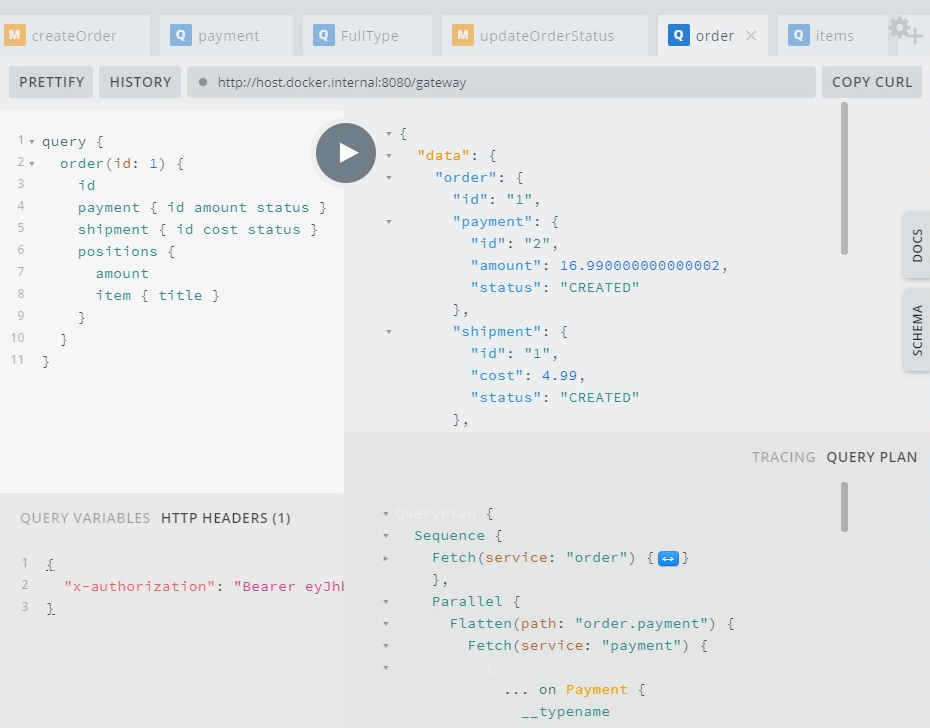
\includegraphics[width=\textwidth]{images/graphql-playground.png}
    \caption{GraphQL Playground Displaying a Query Plan}\label{fig:graphql-playground}
\end{figure}

Apollo Server automatically includes GraphQL Playground, when the gateway is not ran in a production environment.
GraphiQL was included in the microservices using GraphQL and GraphiQL Spring Framework Boot Starters\footnote{\url{https://github.com/graphql-java-kickstart/graphql-spring-boot}}.

\subsubsection{Client Authentication and Authorization}\label{sec:graphql-auth}

Similar to data fetching, which was described in \autoref{sec:graphql-data-fetching}, the more granular control of fields clients want to retrieve requires making authorization of clients more granular too.
The decision of whether or not a client may access certain data must be made on the level of individual fields.

This mechanism was also implemented using \ac{OIDC} via Keycloak and Spring Security as already described in \autoref{sec:rest-auth}.
The injection of data fetchers which was described in \autoref{sec:graphql-data-fetching} into models allows using Spring mechanisms to authorize fetching of certain data.
As an example, \autoref{lst:graphql-auth} shows the fetcher of stock positions of a certain item in the corresponding Spring service.
This method is annotated using Spring Securities annotation, which checks if the authenticated principal of the current request has the role \texttt{inventory\_admin}.

\begin{lstlisting}[caption={Authorization for Retrieval of Individual Fields}, style=java-ext, label={lst:graphql-auth}]
@PreAuthorize("hasRole('inventory_admin')")
public List<ItemStock> lookupItemStockOfItem(long itemId, Integer page, Integer size) {
    return itemStockRepository
            .findAllByItemId(itemId, getPageRequest(page, size))
            .stream()
            .map(this::fromEntity)
            .collect(Collectors.toList());
}
\end{lstlisting}

This separation of authorization logic and the fields an \ac{API} model provides is caused by the Spring Framework itself.
In order to process Java annotations as shown in the listing above, instances of the class need to be created by the framework, which will generate a proxy instance handling the annotated logic at runtime.
Since the instances of model classes are created without a proxy, this feature can not be used directly in place.
However, the usage of fetchers that is required anyways for fields that require complex queries allows to place the authorization logic there.

Using this granular authorization also allows sending partial responses to requests for unauthorized queries.
\autoref{lst:gql-resp-unauthorized} shows a response to an unauthenticated request querying the identifiers of all items and the identifiers of their corresponding stock positions.
Since unauthenticated users are not allowed to obtain any information about stock positions, the \texttt{data} field of the response only includes the identifiers of the items, but returns \texttt{null} for the stock positions.
Additionally, an error is included in the response, specifying which service requires authentication for executing which query.

\begin{lstlisting}[caption={Response to an Unauthorzed Query}, language=json, label={lst:gql-resp-unauthorized}]
{ "errors": [
  { "message": "Access is denied",
    "extensions": { 
      "code": "DOWNSTREAM_SERVICE_ERROR",
      "serviceName": "inventory",
      "query": "{items{id stock{id}}}",
      ...
    }
  }],
  "data": { "items": [ {
    "id": "1",
    "stock": null
  }
}
\end{lstlisting}

\subsubsection{Service-to-Service communication}\label{sec:gql-s2s}

Services of the GraphQL case study communicate only through the federated schema provided by the Federation Gateway as shown in \autoref{sec:graphql-tech}.
This is implemented by passing the \ac{URL} of the gateway to each service.
While the internally exposed GraphQL endpoints of the individual services would be reachable from within the Docker network, the microservices are part of, using the federated schema makes more sense in this case.
In this case, the microservices contribute a part to the overall schema, but are also consumers of the provided \ac{API}.
Even data exposed by the microservice sending the request can be queried in such a query to the gateway.
Using the exposed schemas of the other microservices would have the downside, that multiple queries would need to be sent to different microservices if data of different services was to be obtained and then combined to obtain the required format of the data.

To generate queries, Java classes were generated that resemble the federated schema provided by the gateway using the Ruby Gem \texttt{graphql\_java\_gen} which was already mentioned in \autoref{sec:graphql-tools}.
This tool uses the result of an introspection query to the \ac{API} to generate source code from it.
Apart from instructing the tool to use Java's \texttt{long} primitive type for numerical values and GraphQL identifiers, the tool needs little configuration.
By default, the types \texttt{int} and \texttt{String} would have been used respectively.

Using Java's lambda expressions, the generated code of this tool closely resembles the query language of GraphQL.% checktex 13
An example of updating the status of an order is shown in \autoref{lst:gql-mutation-java}.
In this case, the operation is a mutation with the field \texttt{updateOrderStatus} in its selection set.
The arguments \texttt{orderId} and \texttt{status} are passed to the field and itself has a selection set consisting of the fields \texttt{code}, \texttt{success} and \texttt{message}.

\begin{minipage}{\linewidth}
\begin{lstlisting}[style=java-ext, caption={Formulating Queries against GraphQL \acp{API} using GraphQLJavaGen}, label={lst:gql-mutation-java}]
public void updateOrderStatus(long orderId, OrderStatus status) 
    throws ApiException {
    val query = Operations.mutation(mutation -> mutation
            .updateOrderStatus(orderId, status, response -> response
                    .code()
                    .success()
                    .message()));

    UpdateStatusResponse response = mutate(query).getUpdateOrderStatus();
    if (!response.getSuccess()) {
        throw new ApiException("...");
    }
}
\end{lstlisting}
\end{minipage}

Using this generated code, only means to generate queries and to parse responses are implemented.
The exchange of messages is implemented using Spring's \texttt{RestTemplate} \ac{API}, which was also used to set the required authentication headers in the exchanged \ac{HTTP} messages.
While it would be possible to generate ready-to-use clients, where the transport mechanism is already implemented, using this method makes it easier to use features of the Spring Framework, such as its support for automatically refreshing the required token for authentication.

The clients of the different services only implement the functionality that they require for operation.
In principle, any request can be formulated and any response can be parsed by the generated code, but the services make only use of parts of the schema.
For example, only the client of the order service implements the creation of shipments and payments, while both the payment and shipment service implement updating the status of an order.

\subsection{Architectural Differences of the Implementations}

The following section compares both implementations of the case study based on different aspects.
These aspects were chosen based on the taxonomy of microservices proposed by Garriga~\cite{Garriga2017}, but also based on the experiences of implementing both versions of the case study.
Firstly, the \ac{HTTP} interface of both versions will be compared.
Since both implementations expose their interfaces via \ac{HTTP}, analyzing differences is an important aspect to understand differences in the technologies.
Secondly, the \ac{API} style will be compared.
This aspect is directly related to the interface of the \acp{API}, however, GraphQL can be served over other protocols, so these points were analyzed separately.
Garriga combines these two aspects under the category \textit{Data Exchange}.
Thirdly, the implementation of authentication and authorization will be compared.
This corresponds to the cross-cutting concern \textit{Security} Garriga identified.
Lastly, the concerns \textit{Data Storage}, \textit{Runtime Virtualization} and \textit{Runtime Control Loops} of Garriga's taxonomy will be analyzed in \autoref{sec:comp-data} and \autoref{sec:comp-runtime}.

Because of the limited scope of the case study, other aspects, such as organizational aspects or deployment platform, are not analyzed.
Although these aspects allow for categorizing real world microservice architectures, they are not easily applicable to purely academic case studies.

\subsubsection{\acs{HTTP} Interface}

One of the most striking differences, but also one of the most important properties of the implemented microservices is their \ac{HTTP} interface.
While in both implementations, the microservices expose their interface via \ac{HTTP}, the concrete realization is very different.

While the \ac{REST} services expose an interface, where every resource has its own \ac{URL} and actions on the resources can be controlled via \ac{HTTP} methods, the GraphQL microservices expose one single endpoint each and the action to execute is solely dependent on the \ac{HTTP} body of the request.
As already mentioned in \autoref{sec:graphql-http}, this makes using tools tools and especially caches for \ac{HTTP} difficult, because those typically expect that a resource-based \ac{API} is implemented with \ac{HTTP}.
\ac{HTTP} requests to a GraphQL \ac{API} have just one single \ac{URL} they are requesting, which requires inspecting the request body to be able to cache responses.
Additionally, evaluations about commonly requested entities of the \ac{API} also require deeper inspection of the request body, instead of being able to simply look at the \ac{URL} of the request.

However, clients consuming the \acp{API} are easier to implement using GraphQL.
This is firstly due to the limited set of used features of \ac{HTTP}.
For example, GraphQL by default does not consume any \ac{HTTP} headers because the complete request is contained in the request body.
It uses \ac{HTTP} only to transport data, but not for giving processing instructions.
This drastically differs for \ac{REST} \acp{API}.
The action that should be executed on a resource is specified by the \ac{HTTP} method, often additional query parameters can be passed to a resource, and standard or custom \ac{HTTP} headers are used in requests and responses~\cite{Buelthoff2019}.

Although the \ac{HTTP} interface is so different for both implementations, the server-side code is similar.
This is most likely caused by the overarching Spring framework that was used for both implementations.
Using its plugins Spring \acs{MVC} and GraphQL Spring Boot Starter automatically configure an embedded \ac{HTTP} server and abstract most of the interaction with \ac{HTTP} away.
For the \ac{REST} implementation, Java's annotation can be used to specify which methods should be called when which \ac{URL} is requested.
Variables in the \ac{URL} path, query variables, \ac{HTTP} headers and the request body can be automatically injected as method parameters.
The GraphQL implementation mostly relies on the names of classes and methods to match types and fields in the GraphQL schema with the corresponding classes and methods in Java.
Parameters of GraphQL fields are used in the same order for Java methods.

\subsubsection{\acs{API} Paradigms}

Another important difference between the implemented \acp{API} in the case study is the paradigms they follow.
While \ac{REST} is defined to follow a resource-based style, GraphQL follows a more \ac{RPC}-based style.
As already mentioned in \autoref{sec:rest}, a resource-based style means that the \ac{API} performs operations on so-called resources, which possess one or many representations.
The \ac{RPC} style follows a different approach, by exposing a set of actions --- so-called procedures --- that can be called by the consumer of the \ac{API}.

In the case study, this is implemented by serving representations of the domain objects in \ac{JSON} format for the \ac{REST} \ac{API}.
Additionally, links to related resources are included following the \ac{HAL} format for \ac{JSON}.
The \ac{API} exposed in this way supports only four different kinds of actions.
The \ac{HTTP} \texttt{GET} method can be used to obtain a representation of a domain object, \texttt{POST} creates a new domain object, \texttt{PUT} updates a domain object to match the representation included in the request body, and \texttt{DELETE} deletes a domain object.

While obtaining representations of domain objects can be done in a very similar way in GraphQL by querying either all objects or just one object with a certain identifier, write-operations are implemented very differently than in \ac{REST}.
Each such operation includes a verb indicating the operation to execute, for example \texttt{createItem} or \texttt{updateOrderStatus}.

This makes it clearer, that a server-side procedure is triggered instead of just updating a representation of a domain object.
For example, status updates of orders in the \ac{REST} \ac{API} are implemented by sending a \texttt{PUT} request to a status subresource of an order.
This hides the processing of the shipment domain objects that may be triggered by such an update action from the \ac{API} consumers.

\subsubsection{Authentication and Authorization}

While the previously compared aspects of the implementations have shown quite some differences, authentication could be implemented in the same way for both \ac{REST} and GraphQL.
Both implementations use \ac{OIDC} for authentication, where the user sends a token they obtained from the \ac{IdP} in the \ac{HTTP} \texttt{Authorization} header in the \texttt{Bearer} scheme.
The token is signed by the \ac{IdP} to ensure its integrity and only the signature needs to be validated by the microservices to ensure that a request is authenticated.
Thus, authentication is mostly delegated to the \ac{IdP} Keycloak in both implementations.
The only difference between the implementations is the forwarding to the microservices.
Since the \ac{REST} implementation only uses a reverse-proxy in front of the microservices which does not modify the headers of the requests, the \texttt{Authorization} header is passed through to the microservices as received.
The Apollo Federation Gateway, however, generates new requests from the received requests that are sent to the microservices.
To forward the authentication token to the microservices custom handling of the requests was required to be added to the gateway.
This handler inspects the headers of the request received by the gateway and includes the same value for the \texttt{Authorization} header in the request sent to the upstream microservice.

Although authentication is implemented almost identically in both versions of the case study, authorization is implemented slightly differently.
As explained in \autoref{sec:rest-auth}, authorization in the \ac{REST} implementation of the case study is performed only on complete representations of resources, i.e. if a request is authorized is only decided based on the requested \ac{URL}.
The GraphQL implementation performs authorization on a more granular level by checking authorization on data fetchers (see. \autoref{sec:graphql-auth}).
This means, authorization can be performed for every individual field of every entity of the \ac{API}.
If fields are requested, that the authenticated user is not authorized to fetch, the \texttt{null} value is returned for this field and a corresponding error is included in the response.
In summary, the GraphQL part of the case study implements authorization on a more granular level than the \ac{REST} version.

However, such a granular implementation of authorization could also be implemented in a \ac{REST} \ac{API}.
This would require introducing a similar concept of data fetchers as was implemented in the GraphQL case study.
The models of the \ac{REST} \ac{API} would not contain the concrete values of its fields, but only fetchers for the values which could perform authorization and resolve to a \texttt{null} value if the user is not authorized. 

\subsubsection{Data Storage and Access}\label{sec:comp-data}

Similar to authorization, the same technology was used to implement data storage and access.
Every microservice in both implementations stores its data in a PostgreSQL database, which is shared between all instances of the same microservice.
Although microservice architectures encourage choosing the right database technology for each microservice, in this case, the same database system was chosen because the data model fits in a relational model.

Also data access was implemented in the same way on the lowest level.
Both implementations use Spring Data \ac{JPA} for storing data and querying the database.
However, data access can be controlled on a more granular level with GraphQL.
Using the data fetchers as described in \autoref{sec:graphql-data-fetching}, \ac{API} models can trigger the execution of more complex database queries on demand depending on the requested fields.
In contrast, the \ac{REST} implementation of the case study always executes the same queries to the database depending on the requested resource.

Similar functionality of returning only requested parameters or explicitly specifying related resources that should be included in a response to a request could be implemented in the \ac{REST} case study.
This technique is already implemented in some \ac{REST} \acp{API}\footnote{e.g. the WordPress \ac{API}: \url{https://developer.wordpress.org/rest-api/using-the-rest-api/global-parameters/}}
With such an implementation, a similar interface to that of GraphQL could be implemented and the queries to the database would be dynamically generated based on the requested data of a resource.
However, it would also introduce the downside of a higher probability of cache misses similar to GraphQL.

\subsubsection{Runtime and Deployment}\label{sec:comp-runtime}

While both microservice architectures developed during the case study were not deployed to any real-world environment, comparing the runtime and deployment environments still makes sense because all microservices were bundled ready-for-deployment as container images.
The containers are all based on images of Open\acs{JDK} version 13.
All images of the microservices can be configured by using environment variables.
While some settings can be configured for every microservice, such as the connection settings for the database and \ac{OIDC} client ID and secret, some services require additional configuration.
For example, the GraphQL services requiring access to the exposed data graph also have a setting for the base \ac{URL} of the Federation Gateway.

Using this configuration model, all microservices can be easily deployed as Linux containers, virtual machines, or on bare metal hardware because on every platform environment variables can be easily configured.
However, deploying the microservices as containers also allows for deploying the application on a container orchestration system such as Kubernetes which enables automatic scaling of the microservices.

\subsection{Performance Comparison}

To evaluate the performance of both implementations of the case study, a scenario resembling a burst of orders was simulated.
First, three warehouses, five items, and 13 stock positions distributing stock positions among warehouses for every item are created.
Then 100 orders with up to four positions and between one and three items per position are placed.
The scenario implements a delay between placing orders of zero to 250 milliseconds.
When all orders are placed, the scenario waits for two minutes, to allow for the creation of all dependant resources.
Then the corresponding payments of the created orders are set to status \texttt{paid} to initiate the process of sending out shipments for the orders.
The process of placing the orders, the updates to the statuses of the payments, and the delays are randomly generated, but the same values were used for both parts of the case study.

\begin{figure}[b!]
    \centering
    \begin{tikzpicture}
        \begin{axis}[
            width=\linewidth, % Scale the plot to \linewidth
            height=10cm,
            grid=major, 
            grid style={dashed,gray!30},
            xlabel=Time after Scenario Start, % Set the labels
            ylabel=Average Response Time,
            x unit=s, % Set the respective units
            y unit=ms,
            %legend style={at={(0.5,-0.2)},anchor=north},
            x tick label style={rotate=90,anchor=east},
            ymin=0,
            ymax=200,
            xmin=0,
            xmax=450,
            %extra y ticks={30.5,63.3},
            extra y tick style={
                yticklabel style={font=\footnotesize}
            }
          ]
          \addplot[mark=square*, theme1] table[x=Time,y=REST,col sep=comma] {data/experienced-response-time.csv}; 
          \addlegendentry{REST}
          \addplot[mark=*, theme2] table[x=Time,y=GraphQL,col sep=comma] {data/experienced-response-time.csv}; 
          \addlegendentry{GraphQL}
          \addplot[mark=none, theme1!50!white, dashed] coordinates {(0,30.5) (450,30.5)};
          \addplot[mark=none, theme2!50!white, dashed] coordinates {(0,63.3) (450,63.3)};
        \end{axis}
    \end{tikzpicture}
    \caption{Experienced Average Response Time by Users}\label{fig:exp-resp-time}    
\end{figure}

In total, four different metrics were collected and analyzed to compare the performance.
Firstly, the response time of the services was measured.
Secondly, the number of requests to the services was collected.
Both of these metrics were collected by using the monitoring feature of the reverse proxy software Traefik which was used in both implementations of the case study.
Thirdly, the amount of data received and transmitted by the services was collected.
This metric was obtained by using the Docker plugin for Telegraf\footnote{\url{https://www.influxdata.com/time-series-platform/telegraf/}}, an open-source server agent for collecting metrics.
Using this plugin, the metric is directly collected from the Docker network all services are part of.
This ensures, that only the traffic from and to the services is collected.
Lastly, the number of returned tuples from the database was collected.
This metric can be obtained directly from the employed database system PostgreSQL if the monitoring features are enabled.

Arguably one of the most important metrics for \acp{API} is the average response time the user experiences.
In the case of the case study, this metric can be obtained from the collected data, however, the used data set slightly differs for both implementations of the case study.
For the \ac{REST} implementation, this metric can be seen as the average response time of all services combined, as clients make requests directly to the individual services.
For the GraphQL implementation, however, only the response time of the gateway was used because it receives all external requests and performs additional functions, such as combining query results from individual services to generate a response to a user's query.

The results of this analysis are shown in \autoref{fig:exp-resp-time}.
Requests to the \ac{REST} \ac{API} are almost consistently faster, than to the GraphQL \ac{API}.
The median execution time of requests to the \ac{REST} \ac{API} is 30.5 seconds, whereas the median response time of the GraphQL \ac{API} is more than twice as high at 63.3 seconds.
Both \acp{API} show high initial response times in the beginning between around 600 to 300 seconds.
However, the GraphQL \ac{API} additionally shows outliers in the order of magnitude of one to three seconds which are not plotted in the above figure.

\begin{figure}[h!]
    \centering
    \begin{tikzpicture}
        \begin{axis}[
            width=\linewidth, % Scale the plot to \linewidth
            height=10cm,
            grid=major, 
            grid style={dashed,gray!30},
            xlabel=Time after Scenario Start, % Set the labels
            ylabel=Average Response Time,
            x unit=s, % Set the respective units
            y unit=ms,
            %legend style={at={(0.5,-0.2)},anchor=north},
            x tick label style={rotate=90,anchor=east},
            ymin=0,
            ymax=100,
            xmin=0,
            xmax=450,
            %extra y ticks={21.4,36},
            extra y tick style={
                yticklabel style={font=\footnotesize, xshift=-0.5cm}
            }
          ]
          \addplot[mark=square*, theme1] table[x=Time,y=REST,col sep=comma] {data/order-response-time.csv}; 
          \addlegendentry{REST}
          \addplot[mark=*, theme2] table[x=Time,y=GraphQL,col sep=comma] {data/order-response-time.csv}; 
          \addlegendentry{GraphQL}
          \addplot[mark=none, theme1!50!white, dashed] coordinates {(0,36) (450,36)};
          \addplot[mark=none, theme2!50!white, dashed] coordinates {(0,21.4) (450,21.4)};
        \end{axis}
    \end{tikzpicture}
    \caption{Response Time of the Inventory Service}\label{fig:inventory-resp-time}    
\end{figure}

Surprisingly, when looking at the response time of individual services, this observation differs.
\autoref{fig:inventory-resp-time} shows the response times of the inventory service in the \ac{REST} and GraphQL implementation of the case study.
In this case, the median response time during the scenario lies at 36 seconds for the \ac{REST} service, but only 21.4 seconds for the GraphQL implementation.
However, the measured response time of the GraphQL implementation is not consistently lower than that of the \ac{REST} implementation.
This observation might indicate, that the GraphQL Federation Gateway is a bottleneck in the implementation.

However, the performance of the implementations can not only be measured in the response time of the services but also the number of requests, that must be sent to achieve a goal is an important metric.
Similar to the comparison of response time experienced by the user, to calculate this metric, the number of requests to all services was summed up for the \ac{REST} \ac{API}, while for the GraphQL \ac{API} the number of requests to the gateway was used.
As shown in \autoref{fig:perf-sent-requests}, the cumulated number of requests to the \ac{REST} \ac{API} exhibits a steeper slope than that of the GraphQL implementation.
This was to be expected, as one of GraphQL's main features is being able to formulate queries fetching exactly the required data.
Additionally, the different \ac{API} style allow implementing much more specific functionality as remotely callable procedures as compared to the resource-based \ac{API} implemented by the \ac{REST} \ac{API}.
For example, when booking out items from the inventory, the \ac{REST} \ac{API} requires sending a request for each stock position, where stock is to be removed, while the GraphQL \ac{API} implements a field on its mutation type allowing to book out items from all positions at once.

\begin{figure}[t!]
    \centering
    \begin{tikzpicture}
        \begin{axis}[
            width=\linewidth, % Scale the plot to \linewidth
            height=10cm,
            grid=major, 
            grid style={dashed,gray!30},
            xlabel=Time after Scenario Start, % Set the labels
            ylabel=Received Requests,
            x unit=s, % Set the respective units
            %legend style={at={(0.5,-0.2)},anchor=north},
            legend pos=south east,
            x tick label style={rotate=90,anchor=east},
            ymin=0,
            xmin=0,
            xmax=450
          ]
          \addplot[mark=square*, theme1] table[x=Time,y=REST,col sep=comma] {data/sent-requests.csv}; 
          \addlegendentry{REST}
          \addplot[mark=*, theme2] table[x=Time,y=GraphQL,col sep=comma] {data/sent-requests.csv}; 
          \addlegendentry{GraphQL}
          \addplot[mark=none, theme2!50!white, dashed, shorten >=-2.0cm, thick] table[x=Time,y={create col/linear regression={y=GraphQL}},col sep=comma] {data/sent-requests.csv};
          \addplot[mark=none, theme1!50!white, dashed, shorten >=-2.0cm, thick] table[x=Time,y={create col/linear regression={y=REST}},col sep=comma] {data/sent-requests.csv};

        \end{axis}
    \end{tikzpicture}
    \caption{Cummulated Received Requests in the System}\label{fig:perf-sent-requests}    
\end{figure}


\begin{figure}[t!]
    \centering
    \begin{tikzpicture}
        \begin{axis}[
            width=\linewidth, % Scale the plot to \linewidth
            height=10cm,
            grid=major, 
            grid style={dashed,gray!30},
            xlabel=Time after Scenario Start, % Set the labels
            ylabel=Received Data,
            x unit=s, % Set the respective units
            y unit=kB,
            %legend style={at={(0.5,-0.2)},anchor=north},
            legend pos=south east,
            x tick label style={rotate=90,anchor=east},
            ymin=0,
            xmin=0,
            xmax=450
          ]
          \addplot[mark=square*, theme1] table[x=Time,y=REST,col sep=comma] {data/kb-received.csv}; 
          \addlegendentry{REST}
          \addplot[mark=*, theme2] table[x=Time,y=GraphQL,col sep=comma] {data/kb-received.csv}; 
          \addlegendentry{GraphQL}
          \addplot[mark=none, theme2!50!white, dashed, shorten >=-2.0cm, thick] table[x=Time,y={create col/linear regression={y=GraphQL}},col sep=comma] {data/kb-received.csv};
          \addplot[mark=none, theme1!50!white, dashed, shorten >=-2.0cm, thick] table[x=Time,y={create col/linear regression={y=REST}},col sep=comma] {data/kb-received.csv};

        \end{axis}
    \end{tikzpicture}
    \caption{Cummulative Amount of Data Received by the Services}\label{fig:perf-sent-data}    
\end{figure}

As can be expected based on these findings, also the amount of data transferred over the network is higher when using the \ac{REST} \ac{API} than when using the GraphQL implementation.
This measurement includes the amount of received data by all containers in one implementation, so for the \ac{REST} implementation, it includes the traffic to the reverse proxy and the forwarded request from the reverse proxy to the service.
Similarly, the measurement for the GraphQL implementation includes queries to the gateway and the subqueries it generates for the services.
Based on the resulting graph shown in \autoref{fig:perf-sent-data}, the received requests by the services and the received data seem to correlate almost linearly.
However, the amount of received data also increases slightly, when no requests were received.
This is caused by network activities other than the scenario.
For example, the Docker containers of the microservices regularly run a health-check for the service which does not use the reverse-proxy and thus can not be observed by the received requests metric.
Additionally, the traffic that the containers cause by using regular functionality of the operating system, for example \ac{DNS} queries, is attributed to them in this metric.


\begin{figure}[t!]
    \centering
    \begin{tikzpicture}
        \begin{axis}[
            width=\linewidth, % Scale the plot to \linewidth
            height=10cm,
            grid=major, 
            grid style={dashed,gray!30},
            xlabel=Time after Scenario Start, % Set the labels
            ylabel=Returned Tuples,
            x unit=s, % Set the respective units
            %y unit=kB,
            %legend style={at={(0.5,-0.2)},anchor=north},
            legend pos=south east,
            x tick label style={rotate=90,anchor=east},
            ymin=0,
            ymax=280000,
            xmin=0,
            xmax=450,
            scaled ticks=false,
            tick label style={/pgf/number format/fixed}
            ]
            \addplot[mark=square*, theme1] table[x=Time,y=REST,col sep=comma] {data/returned-tuples.csv}; 
            \addlegendentry{REST}
            \addplot[mark=*, theme2] table[x=Time,y=GraphQL,col sep=comma] {data/returned-tuples.csv}; 
          \addlegendentry{GraphQL}
          \addplot[mark=none, theme2!50!white, dashed, shorten >=-2.0cm, thick] table[x=Time,y={create col/linear regression={y=GraphQL}},col sep=comma] {data/returned-tuples.csv};
          \addplot[mark=none, theme1!50!white, dashed, shorten >=-2.0cm, thick] table[x=Time,y={create col/linear regression={y=REST}},col sep=comma] {data/returned-tuples.csv};

        \end{axis}
    \end{tikzpicture}
    \caption{Cummulated Tuples Returned by Database Queries}\label{fig:perf-tuples}    
\end{figure}

Another surprising observation is the fact, that the \ac{REST} microservices cause a higher load on the database system than the GraphQL services.
\autoref{fig:perf-tuples} shows the cumulated amount of returned tuples by the database system.
The number of requests for the \ac{REST} \ac{API} is steeper than that of the GraphQL \ac{API}, with a difference of around 50.000 returned tuples after the scenario executed.
This is surprising because the resource-based \ac{API} style of \ac{REST} usually only reads very few database entities.
GraphQL, however, can be used to formulate arbitrarily complex queries spanning multiple entities and multiple services, which was expected to cause more tuples to be read from the database.
Similar to the received data, this metric is slightly skewed by the observation itself.
As mentioned before, the returned tuples are a metric that can be obtained from the PostgreSQL database system if monitoring features are enabled.
The collected metrics then can be queried from a special database, where queries also return tuples which are then included in the metric.

\subsection{Schema Evolution}

To address research question 3, the schema of both implementations of the case study was intentionally evolved.
In the first implementation, the cost of shipments was constant.
After the evolution, all items are supposed to include an additional field for the weight of an item.
The shipping cost then is dependant on the total weight of the order.

As a first step, the database model of both inventory services was changed.
Since both the \ac{REST} and GraphQL implementation use \ac{JPA} as their persistence layer, this modification is the same in both services.
\autoref{lst:schema-ext} shows the required modification on the item database entities to allow storing a weight.

\begin{lstlisting}[style=java-ext, caption=Extended Database Schema of Items, label=lst:schema-ext]
@Column(nullable = false)
private double weight;
\end{lstlisting}

The next step was to expose this value in the database in the provided \acp{API}.
For the \ac{REST} implementation, it was sufficient to add a field in the \ac{API} model and copy the value, when the model is created from a database entity.
\autoref{lst:api-model-ext} shows the extended \ac{API} model.
Since the models already contained annotations describing how models should be parsed from \ac{JSON} and how field values should be validated, no further modification of an \ac{API} controller was needed.

\begin{minipage}{\linewidth}
\begin{lstlisting}[style=java-ext, caption=Extended \ac{API} Model for Items in the \ac{REST} Inventory Microservice, label=lst:api-model-ext]
@Getter
@EqualsAndHashCode(callSuper = true)
public class Item extends RepresentationModel<Item> {
    // [...]
    @PositiveOrZero
    private final double weight;
    
    @JsonCreator
    public Item(// [...],
                @JsonProperty("weight") double weight) {
        // [...]
        this.weight = weight;
    }
    public static Item from(ItemEntity entity) {
        Item item = new Item(/* [...], */ entity.getWeight());
        return item;
    }
}
\end{lstlisting}
\end{minipage}

The GraphQL implementation needed more changes to add the additional field in the inventory microservice.
First of all, the schema definition needed adaption to include the additional field \texttt{weight} for the item type, but additionally the corresponding mutation field \texttt{createItem} needed the same value as a parameter.
Since GraphQL only allows scalar values or input types to be used as parameters (see \autoref{sec:graphql-schemas}), this could not be realized as a single type, like for the \ac{REST} implementation.
While similar changes to the \ac{API} model class were needed as for \ac{REST}, the schema changes also needed to be reflected in the Java class corresponding to the mutation type.

Although the implementation of the schema modification in the inventory service was more complex for the GraphQL version of the case study, the consuming part of the application could be implemented very easily in the shipment service.
The first step was to regenerate the client code as described in \autoref{sec:gql-s2s}.
With the new fields available in the client \ac{API}, a query as shown in \autoref{lst:rq3-query} can be formulated to calculate the total weight of an order given its identifier.

\begin{lstlisting}[style=java-ext, caption=Querying the Total Weight of an Order using GraphQL, label=lst:rq3-query]
public double getOrderWeight(long orderId) throws ApiException {
    val query = Operations.query(q -> q
            .order(orderId, order -> order
                    .positions(position -> position
                            .amount()
                            .item(item -> item
                                    .weight()))));
    Order order = this.query(query).getOrder();
    return order.getPositions().stream()
        .mapToDouble(p -> p.getAmount() * p.getItem().getWeight())
        .sum();
}
\end{lstlisting}

Using this query, the calculation of the shipping cost could be replaced with a mapping of the weight of the order to a price instead of using a constant.
Because it is possible to calculate the total weight of an order using just one query --- which is broken down to one subquery to the order and one to the inventory microservice, --- the GraphQL implementation does not store the weight of the order but queries it every time it is required.

This differs from the \ac{REST} implementation.
If the weight of an order would be calculated only when it is required, first a request to the order service would be required to obtain the positions of the order, and then one request for every position to the inventory microservice would be required.
Due to this overhead, the order microservice additionally stores the weight of the item for each position.
To achieve this, first, the \ac{API} client for the inventory service needed to be adapted in the order microservice, then the model of the database entity for order positions needed to adapted similar to \autoref{lst:schema-ext}.
The \ac{API} model then was extended with a field that is not required for the creation of an order, but is included in order resources when they are returned to the client.
Filling this value requires an additional database query every time an order is requested.

Finally, the client for the order \ac{API} could be updated in the shipping microservice to be able to fetch the weight of orders.
When the cost of a shipment is requested from the shipment \ac{API}, a request to the order microservice is sent to determine the weight of the order.
Based on this value, the price for the shipment can be determined as was described for the \ac{REST} implementation.

\subsection{Discussion}

This case study shows that there can not be a clear recommendation of GraphQL or \ac{REST} over the other for implementing microservice architectures.
The results of the comparison show that the differences between implementing microservices with both these interface technologies are, in fact, minor.
While the style of the \acp{API} and the \ac{HTTP} interfaces the services expose follows very different paradigms, the actual implementation of the microservices followed a very similar architectural style.
Also the performance measurements could not reveal a clear recommendation of one technology.
While the \ac{REST} implementation exhibits a faster overall response time over the GraphQL implementation, the fact that the same task could be performed with significantly less requests overall is not negligible.
The only aspect, where GraphQL performed better over \ac{REST} was the schema evolution which was introduced as part of (RQ3).
While the modification of the \ac{API} required changes in more places in the source code, the consuming \ac{API} client could be implemented very conveniently.

Based on the results of the compared aspects of both implementations, both implementations have advantages in different categories.
This implies that the technology selection for implementing interfaces in microservices relies heavily on preference instead of clear technological superiority.
The higher response time of the GraphQL Federation Gateway over the \ac{REST} \ac{API} is probably acceptable in most scenarios because the total number of requests is also significantly smaller in order to achieve the same goal.
The finding that implementing the \ac{API} client of GraphQL requires less effort than implementing a \ac{REST} client is in accordance with the findings of Brito~\cite{Brito2020}.

However, this thesis and its results also have several limitations.
Firstly, a typical case study requires multiple sources of evidence and a triangulation of the insights gained from the sources~\cite{Runeson2012}.
The only aspect that was triangulated in this thesis is the methodology.
Research question (RQ1) and (RQ3) used mostly qualitative methods, while (RQ2) was based on quantitative data.
However, only the implemented case study was used as a data source and the observation was only performed by the author.
Secondly, both versions of the case study used the Spring Framework as their foundation.
While this framework is very commonly used among developers, the results of the analysis is also dependant on the usage of it.
Using no framework or different frameworks might show different results and especially different results for the performance measurements.
Lastly, the collected data of (RQ2) contains the negative impact of running the microservices in containers~\cite{Kratzke2017}.
While the data is assumed to be comparable, as both versions of the case study was run in containers, especially the response time metric includes the performance impact introduced by containers.
